% DEPRECATED !!! %

\subsection{Type Library Plugin}

The DSL has to support custom datatypes like \texttt{Money}, which must be
defined somewhere. We could define them in the user projects, but it is better
to offer them as a library. Later, our code generator needs also needs to know
how to map these types to widgets, which we will also add to the library.

Thus, we will create now a library project. Open the New Project wizard (\emph{File /
New Project}) and choose \emph{Plug-in Project} from the \emph{Plug-in Development} category.

On the first page, enter the project's name: \emph{org.eclipse.xtext.example.ql.lib}.

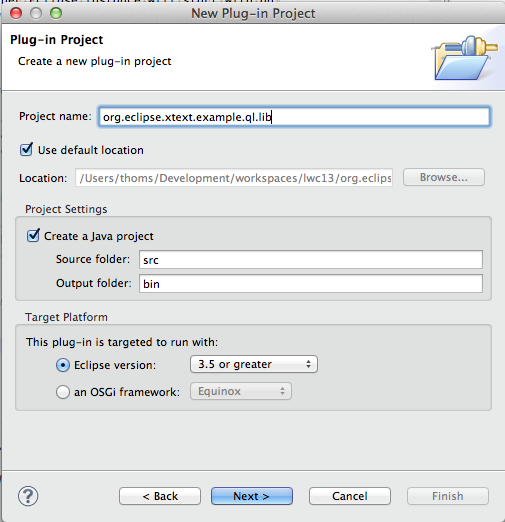
\includegraphics[width=10cm]{./images/chapter01/NewPluginProject_01.png}

Press \emph{Next}. On the second page, uncheck the options \emph{``Generate an
activator\ldots''} and \emph{``This plug-in will make contributions to the UI''}.

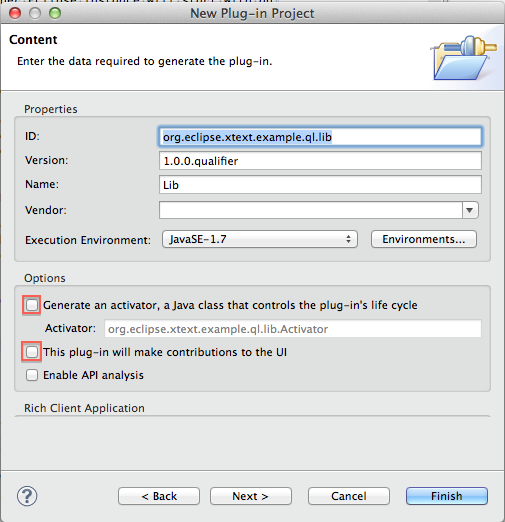
\includegraphics[width=10cm]{./images/chapter01/NewPluginProject_02.png}

Press Finish to create the project now.

Select the \texttt{/src} folder and create a new Java class \texttt{Money} in package
\texttt{types}:
\begin{lstlisting}[language=Java]
package types;

import java.math.BigDecimal;

public class Money {
  private BigDecimal amount;

  public Money(BigDecimal amount) {
    this.amount = amount;
  }

  public BigDecimal getAmount() {
    return amount;
  }
}
\end{lstlisting}

Now open \texttt{META-INF/MANIFEST.MF} and go to the Runtime page. To make the type
visible later, we have to declare that the \texttt{types} package is exported. Click the
\emph{Add} button and select the \texttt{types} package.

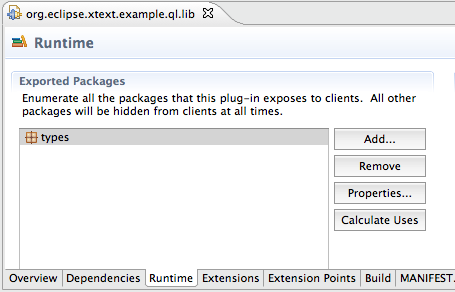
\includegraphics[width=10cm]{./images/chapter01/ExportPackage.png}

If you want to support any further custom datatype, just add them as new classes
to the types package.

